\documentclass[amsmath,superscriptaddress,showpacs,aps,prb,twocolumn]{revtex4-1}
\usepackage[colorlinks,linkcolor=blue,anchorcolor=blue,citecolor=blue,urlcolor=blue]{hyperref}
\usepackage{amsmath}
\usepackage{amssymb}
\usepackage{graphicx}
\usepackage{color}
\usepackage{bm}

\begin{document}
\title{Flatband ferromagnetism and dispersion relations of spin-1 excitations in topological Hubbard models}
\author{Xiao-Fei Su}
\affiliation{National Laboratory of Solid State Microstructures and Department of Physics, Nanjing University, Nanjing 210093, China}
\affiliation{School of Physics and Electronic Information, Huaibei Normal University, Huaibei 235000, China}
\author{Zhao-Long Gu}
\affiliation{National Laboratory of Solid State Microstructures and Department of Physics, Nanjing University, Nanjing 210093, China}
\author{Zhao-Yang Dong}
\affiliation{National Laboratory of Solid State Microstructures and Department of Physics, Nanjing University, Nanjing 210093, China}
\author{Shun-Li Yu}
\affiliation{National Laboratory of Solid State Microstructures and Department of Physics, Nanjing University, Nanjing 210093, China}
\affiliation{Collaborative Innovation Center of Advanced Microstructures, Nanjing University, Nanjing 210093, China}
\author{Jian-Xin Li}
\affiliation{National Laboratory of Solid State Microstructures and Department of Physics, Nanjing University, Nanjing 210093, China}
\affiliation{Collaborative Innovation Center of Advanced Microstructures, Nanjing University, Nanjing 210093, China}
\date{\today}

\begin{abstract}
\par We study the spin-1 excitation spectra of the flatband ferromagnetic phases in topological Hubbard models. As a paradigm, we consider a quarter filled square lattice Hubbard model whose free part is the $\pi$ flux model with topologically nontrivial and nearly-flat electron bands. The model Hamiltonian either explicitly breaks the time-reversal symmetry but preserves the spin $SU(2)$ rotation symmetry (Chern Hubbard model), or preserves the time-reversal symmetry but explicitly breaks the spin $SU(2)$ rotation symmetry ($Z_2$ Hubbard model). By using the numerical exact diagonalization method with a projection onto the lower nearly-flat electron band, we determine the critical Hubbard interaction strength upon which the ferromagnetic phase is stable, and elaborate the ferromagnetic spin-1 excitation spectra of the Chern Hubbard model and the $Z_2$ Hubbard model. Both spectra consist of collective modes (spin waves) and individual modes (Stoner continuum). For the Chern Hubbard model, the spin wave is gapless while for the $Z_2$ Hubbard model, the spin wave is gapped. Remarkably, for both cases, the nonflatness of the free electron bands introduces dips of the lower boundary of the Stoner continuum, \textcolor{red}{and the scatterings between the Stoner continuum at these dips and the collective modes significantly reduce the latter's energy}, which can lead to roton-like spin wave excitations. With the increase of this nonflatness, the energy of the induced roton-like modes goes down and finally touches zero, which results in the destabilization of the ferromagnetic phase.
\end{abstract}
\maketitle

\section{Introduction}
\par Electronic bands with nonzero topological indices reside on the center of a substantial amount of topological phenomena in condensed matter physics \cite{HK_RMP2010,QZ_RMP2011}. It was proposed in a pioneering work by Haldane \cite{H_PRL1988} that a spinless fermionic model on a honeycomb lattice exhibits integer quantum Hall effect \cite{KDP_PRL1980} without an external magnetic field. This model, serving as the first example of Chern insulator, breaks the time reversal symmetry with a complex next nearest neighbor hopping and is characterized by a nonzero Chern number \cite{TKNN_PRL1982}. Later, the concept was generalized to time reversal symmetric systems with spin-orbital coupling (SOC), such as the monolayer graphene \cite{KM_PRL2005a,KM_PRL2005b} and HgTe/CdTe quantum wells \cite{BHZ_S2006,Ketc_S2007}. The SOC there generates complex hopping terms similar to that proposed by Haldane but with opposite chiralities for electrons with up spins and down spins, resulting in the quantum spin Hall insulator characterized by a $Z_2$ index.

\par The lattice models with nontrivial band topology share much similarity with the two-dimensional electron gas (2DEG) under a strong magnetic field with Landau levels, e.g. the existence of topologically protected gapless edge states \cite{H_PRL1988,L_PRB1981,H_PRB1982,KM_PRL2005a,KM_PRL2005b,BHZ_S2006,Ketc_S2007}. Thus more novel phases other than the Chern insulator or $Z_2$ insulator are expected when Coulomb interactions are taken into account, as is similar to the fractional quantum Hall effect \cite{TSG_PRL1982,L_PRL1983} in the 2DEG with Landau levels. However, different from Landau levels, energy bands in lattice models usually have noneligible dispersions, which weakens the effect of Coulomb interactions. Therefore, in recent years, much effort has been devoted to the design and search of tight-binding models that host nearly-flat electron bands with nontrivial topology \cite{TMW_PRL2011,WR_PRB2011,SGKD_PRL2011,WGGS_PRL2011,NSCM_PRL2011,TB_PRB2012,YGSD_PRB2012}. Analogous exotic phases, such as the fractional Chern insulator and fractional topological insulator were numerically verified to emerge in such nearly-flat topological bands when strong Coulomb interactions are turned on \cite{NSCM_PRL2011,SGSS_NC2011,RB_PRX2011,NSRCM_PRB2011,LBFL_PRL2012}.

\par Another involved intriguing phenomenon arising from Coulomb repulsions in flat or nearly-flat bands is the itinerant ferromagnetism \cite{T_PTP1998}. It was proved by Tasaki and Mielke that the ground state of an flat electron band with its filling factor not more than but sufficiently close to $1/2$ is ferromagnetically ordered as long as an infinitesimal onsite Hubbard repulsion is present \cite{T_PRL1992,M_PLA1993,MT_CMP1993}. Afterwards this ferromagnetism was shown to be stable against small nonflatness of the electron bands if and only if the Hubbard interaction exceeds a critical value \cite{T_PRL1994}. Spin wave excitations over this ferromagnetic ground state was also studied \cite{KA_PRL1994,SGDL_arXiv2008} and itinerant topological magnons has been reported quite recently \cite{SGDL_arXiv2008}.

\par The interplay between flatband ferromagnetism and nontrivial band topology enriches the related physics. In fact, ferromagnetism is essential in the generation of stable fractional Chern insulators in the proposals where the spin degrees of freedom of electrons are considered \cite{TMW_PRL2011,NSRCM_PRB2011,LBFL_PRL2012}. Furthermore, ferromagnetism can also lead to possible high-temperature quantum anomalous Hall effect (QAHE) when the nearly-flat topological band is half-filled \cite{NSRCM_PRL2012}. In this paper, we focus on this ferromagnetism induced QAHE in nearly-flat topological bands. As a paradigm, we consider a square lattice Hubbard model whose free part is the $\pi$ flux model with topologically nontrivial and nearly-flat electron bands. The model Hamiltonian either explicitly breaks the time-reversal symmetry but preserves the spin $SU(2)$ rotation symmetry (Chern Hubbard model), or preserves the time-reversal symmetry but explicitly breaks the spin $SU(2)$ rotation symmetry ($Z_2$ Hubbard model). When the model is quarter filled (or correspondingly, the lower nearly-flat band is half filled), the ground state is spin fully polarized due to the ferromagnetism and exhibits QAHE because of the nonzero Chern number of a single-spin band. Then the low energy physics is dominated by the one-spin-flip excitations. These spin-1 excitations has been studied by a generalized bosonization scheme where the interacting fermionic model is mapped to a free bosonic model describing spin-wave excitations at the harmonic approximation \cite{DG_PRB2015}. The ferromagnetism was shown to be stable against such spin wave excitations, which are gapless in the Chern Hubbard model and gapped in the $Z_2$ Hubbard model. However in this bosonization scheme, the free part of the electron model plays no role in the spin wave excitations other than contributing a global constant, which means it should fail due to the competition between the kinetic energy and potential energy of electrons when the nonflatness of the electron bands is not negligible \cite{T_PRL1994}. What's worse, in a strictly local periodic tight-binding model, an energy band with a nonzero Chern number cannot be exactly flat \cite{CMST_JPMT2014}. Therefore it remains an open question on whether the ground state is stable against the spin-1 excitations and how the the nonflatness of the electron bands manifests itself in the spin-1 excitation spectra in such models.

\par To elucidate these questions, we adopt the numerical exact diagonalization method with a projection onto the lower nearly-flat band to take close investigations on the spin-1 excitations of the models. A critical Hubbard interaction strength is found for both the Chern Hubbard model and the $Z_2$ Hubbard model, upon which the ferromagnetic phase is stable. Furthermore the spin-1 excitation spectra are shown to consist of collective modes (spin waves) and individual modes (Stoner continuum). For the Chern Hubbard model, the spin wave is gapless while for the $Z_2$ Hubbard model, the spin wave is gapped. Remarkably, for both cases, the nonflatness of the free electron bands introduces dips of the lower boundary of the Stoner continuum, \textcolor{red}{and the scatterings between the Stoner continuum at these dips and the collective modes significantly reduce the latter's energy}, which can lead to roton-like spin wave excitations. With the increase of this nonflatness, the energy of the induced roton-like modes goes down and finally touches zero, which results in the destabilization of the ferromagnetic phase.

\par The rest of the paper is organized as follows. In Sec. \ref{mm}, we introduce the Chern Hubbard model and $Z_2$ Hubbard model studied in this paper, discuss the nontrivial band topology of their free parts, interpret the emergence of QAHE resulting from the interplay of flat-band ferromagnetism and nontrivial band topology, and formulate the exact diagonalization method with a projection onto the lower nearly-flat band on details. In Sec. \ref{nr}, we summarize the phase diagram and elaborate the spin-1 excitation spectra of both models. Section \ref{sd} provides a summary and discussion.

\section{Model and method}\label{mm}
\subsection{Introduction to model}\label{intro_to_model}

\begin{figure}
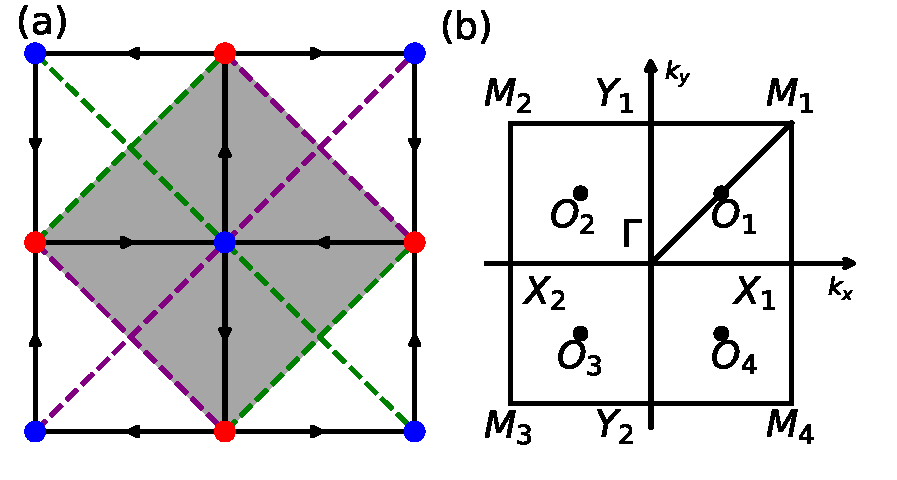
\includegraphics[width=\columnwidth]{lattice}
\caption{(Color online) (a) Schematic representation of the $\pi$-flux model. Blue and red solid circles denote the $A$ and $B$ sublattices, respectively. The nearest-neighbor hopping amplitudes (solid black lines) are equal to $t_{1}\exp[i\alpha(\sigma)\pi/4]$ ($\alpha(\sigma)=1$ for the time-reversal-symmetry-breaking case and $\alpha(\sigma)=\pm1$ for the time-reversal-symmetry-preserving case) along the direction of the arrows, the next-nearest-neighbor hopping amplitudes are equal to $t_{2}$ (dashed green lines) and $-t_{2}$ (dashed purple lines). The shaded area denotes the unit cell. (b) First Brillouin Zone. $\Gamma=(0,0)$, $X_{1,2}=(\pm\pi,0)$, $Y_{1,2}=(0,\pm\pi)$, $M_{1,2,3,4}=(\pm\pi,\pm\pi)$.}
\label{lattice}
\end{figure}

\par We consider a generalized $\pi$-flux Hubbard model on the square lattice, whose Hamiltonian can be written as $H=H_0+H_U$, where $H_0$ is the generalization with electron spin of the original spinless model proposed in Ref. \cite{NSCM_PRL2011},
\begin{equation}
H_0=\sum_{\langle ij\rangle,\sigma}(t_1^{ij,\sigma}c_{i\sigma}^\dagger c_{j\sigma}+\text{H.c.})
    +\sum_{\langle\langle ij\rangle\rangle,\sigma}(t_2^{ij}c_{i\sigma}^\dagger c_{j\sigma}+\text{H.c.}),
\end{equation}
and $H_U$ is the Hubbard interaction
\begin{equation}
H_U=U\sum_{i}n_{i\uparrow}n_{i\downarrow}.
\end{equation}
Here, $c_{i\sigma}^{\dagger}(c_{i\sigma})$ creates (annihilates) a spin $\sigma$ electron at site $i$, $n_{i\sigma}$ is the spin $\sigma$ electron number operator at site $i$, $\langle ij\rangle$ denotes the nearest-neighbor (NN) bonds and $\langle\langle ij\rangle\rangle$ denotes the next-nearest-neighbor (NNN) bonds. As is shown in Fig. \ref{lattice}(a), the spin-dependent NN hopping amplitude $t_1^{ij,\sigma}$ and the spin-independent NNN hopping amplitude $t_2^{ij}$ are given by
\begin{equation}
t_1^{ij,\sigma}=t_1\exp\left[i(-1)^{\delta^1_{ij}}\alpha_\sigma\pi/4\right],
\end{equation}
\begin{equation}
t_2^{ij}=t_2(-1)^{\delta^2_{ij}}.
\end{equation}
Here, $\delta^1_{ij}=+1$ if the NN electron hopping is along the direction of the solid black arrow and $\delta^1_{ij}=-1$ if along the reversed direction. $\delta^2_{ij}=+1$ if the NNN electron hopping is along the dashed green lines and $\delta^2_{ij}=-1$ if along the dashed purple lines. The spin-dependent phase $\alpha_\sigma$ breaks the time-reversal symmetry but preserves the spin $SU(2)$ rotation symmetry if $\alpha_\uparrow=\alpha_\downarrow=+1$, whereas it preserves the time-reversal symmetry but breaks the spin $SU(2)$ rotation symmetry if $\alpha_\uparrow=+1$ and $\alpha_\downarrow=-1$.

\par Due to the complex NN hopping, each electron will acquire a $\pi$ phase as it hops around a plaquette along the direction of the black arrows as indicated in Fig. \ref{lattice}(a). Therefore, $H_0$ describes free electrons hopping on a square lattice in the presence of a fictitious staggered $\pi$-flux pattern \cite{WWZ_PRB1989}. For the time-reversal-symmetry-breaking case, $\alpha_\uparrow=\alpha_\downarrow$, the flux experienced by spin-up electrons and spin-down electrons is the same, while for the time-reversal-symmetry-preserving case, $\alpha_\uparrow=-\alpha_\downarrow$, it is opposite.

\subsection{Topology of free part}\label{topo_free_part}
\par Gapped noninteracting fermionic systems can be topologically classified in the presence of symmetries by their Hamiltonians in the momentum space\cite{SRFL_PRB2008}. After the Fourier transformation, the free part $H_0$ of our model reads
\begin{equation}
H_0=\sum_{\mathbf{k}\sigma}\psi^{\dagger}_{\mathbf{k}\sigma}h_{\mathbf{k}\sigma}\psi_{\mathbf{k}\sigma},
\end{equation}
where $\psi^{\dagger}_{\mathbf{k}\sigma}=(c^{\dagger}_{A\mathbf{k}\sigma},c^{\dagger}_{B\mathbf{k}\sigma})$ and
\begin{equation}
h_{\mathbf{k}\sigma}={\mathbf{D}_{\mathbf{k}\sigma}}\cdot\bm{\tau}.
\end{equation}
Here $\bm{\tau}=(\tau_{1},\tau_{2},\tau_{3})$ is a $2\times2$ matrix vector, $\tau_{1},\tau_{2},\tau_{3}$ are the three Pauli matrices for the sublattice degrees of freedom. The components of $\mathbf{D}_{\mathbf{k}\sigma}$ are given by
\begin{equation}
\begin{aligned}
&D_{1,\mathbf{k}}=2\sqrt{2}t_{1}\cos\frac{k_{x}}{2}\cos\frac{k_{y}}{2},\\
&D_{2,\mathbf{k}}=2\sqrt{2}t_{1}\alpha_\sigma\sin\frac{k_{x}}{2}\sin\frac{k_{y}}{2},\\
&D_{3,\mathbf{k}}=2t_{2}(\cos k_{x}-\cos k_{y}).
\end{aligned}
\end{equation}
$H_0$ can be diagonalized with the transformation
\begin{equation}
\begin{aligned}
&c_{A\mathbf{k}\sigma}=\mu_{1,\mathbf{k}\sigma}d_{\mathbf{k}\sigma}+\mu_{2,\mathbf{k}\sigma}f_{\mathbf{k}\sigma},\\
&c_{B\mathbf{k}\sigma}=\mu^{\ast}_{1,\mathbf{k}\sigma}f_{\mathbf{k}\sigma}-\mu^{\ast}_{2,\mathbf{k}\sigma}d_{\mathbf{k}\sigma},\\
\end{aligned}
\end{equation}
where
\begin{equation}
\begin{aligned}
&\mu_{1,\mathbf{k}\sigma}=\frac{D_{1,\mathbf{k}}-i\alpha_\sigma D_{2,\mathbf{k}}}{\sqrt{2D_{\mathbf{k}}(D_{\mathbf{k}}+D_{3,\mathbf{k}})}},\\
&\mu_{2,\mathbf{k}\sigma}=\frac{D_{\mathbf{k}}+D_{3,\mathbf{k}}}{\sqrt{2D_{\mathbf{k}}(D_{\mathbf{k}}+D_{3,\mathbf{k}})}},\\
\end{aligned}
\end{equation}
with $D_{\mathbf{k}}=\sqrt{D^2_{1,\mathbf{k}}+D^2_{2,\mathbf{k}}+D^2_{3,\mathbf{k}}}$. The diagonalized $H_0$ is given by
\begin{equation}
H_{0}=\sum_{\mathbf{k}\sigma}\varepsilon_{d}(\mathbf{k})c^{\dagger}_{\mathbf{k}\sigma}c_{\mathbf{k}\sigma}
      +\sum_{\mathbf{k}\sigma}\varepsilon_{f}(\mathbf{k})f^{\dagger}_{\mathbf{k}\sigma}f_{\mathbf{k}\sigma},
\end{equation}
where $\varepsilon_{d}(\mathbf{k})=-D_{\mathbf{k}}$, $\varepsilon_{f}(\mathbf{k})=D_{\mathbf{k}}$. It can be seen that there exists a gap between the $d$ band and $f$ band when $t_1\ne0$ and $t_2\ne0$.
\par When there is a gap between the $d$ band and the $f$ band, these bands can be shown to be topologically non-trivial by calculating their Chern numbers \cite{TKNN_PRL1982} (for the time-reversal-symmetry breaking case) or $Z_2$ indices \cite{KM_PRL2005b,SWSH_PRL2006} (for the time-reversal-symmetry preserving case). The Chern number for a single spin component of the $d$ band or the $f$ band can be expressed in terms of the coefficients $D_{i,\mathbf{k}}$ \cite{HK_RMP2010,QZ_RMP2011},
\begin{equation}
C_{\sigma}^{d/f}=\pm\frac{1}{4\pi}\int_{BZ}d^{2}k\;
    \hat{\mathbf{D}}_{\mathbf{k}\sigma}\cdot(\partial_{k_{x}}\hat{\mathbf{D}}_{\mathbf{k}\sigma}\times\partial_{k_{y}}\hat{\mathbf{D}}_{\mathbf{k}\sigma})
    =\pm\alpha_\sigma,
\end{equation}
with $\hat{\mathbf{D}}_{\mathbf{k}\sigma}\equiv\mathbf{D}_{\mathbf{k}\sigma}/D_{\mathbf{k}}$.
\par When the system breaks the time-reversal symmetry, i.e. $\alpha_\uparrow=\alpha_\downarrow=1$, $C_\uparrow^d=C_\downarrow^d=1$ and $C_\uparrow^f=C_\downarrow^f=-1$, the total Chern number of the $d$ band is $C^d=C_\uparrow^d+C_\downarrow^d=2$. Therefore, the ground state of $H_0$ will be a noninteracting Chern insulator and exhibits quantum anomalous Hall effect(QAHE) when the lower $d$ band is fully filled. When the system preserves the time-reversal symmetry, i.e. $\alpha_\uparrow=-\alpha_\downarrow=1$, $C_\uparrow^d=-C_\downarrow^d=1$ and $C_\uparrow^f=-C_\downarrow^f=-1$, the total Chern number of the $d$ band is zero. However, the $Z_2$ index, which is defined as
\begin{equation}
\nu=\frac{1}{2}(C_{\uparrow}-C{\downarrow})\mod2,
\end{equation}
of the $d$ band is $1$ and nontrivial. As a consequence, the the ground state of $H_0$ will be a noninteracting $Z_2$ insulator and exhibits quantum spin Hall effect(QSHE) when the lower $d$ band is fully filled.

\subsection{Emergence of QAHE in half-filled nearly-flat topological bands}\label{emerg_qahe}
\par For a free fermionic system hosting an energy band with a nonzero Chern number or $Z_2$ index, the distinguished phenomenon resulting from this nontrivial band topology, such as QAHE or QSHE, only manifests itself when the topological band is fully filled. At any fractional filling, the ground state of such a system will be a trivial metal. Intriguingly, when the Coulomb interactions between electrons step in, the physics of the nontrivial band topology becomes more involved, especially when the band is nearly flat so that the effects of the Coulomb interactions are highly enhanced. Combined with strong Coulomb interactions, nontrivial topological phases can emerge from fractionally filled topological bands. In this article, we are interested in half-filled strongly-correlated nearly-flat topological bands where QAHE can arise\cite{NSCM_PRL2011,DG_PRB2015}. The essence for the occurrence of this nontrivial phase is the emergence of itinerant ferromagnetism on nearly-flat bands\cite{T_PTP1998}, which fully polarizes all the electron spins. Therefore only one spin component of the topological band will be fully filled exactly, which leads to QAHE due to the nonzero Chern number of that spin component of the band.

\par The Chern Hubbard model and $Z_2$ Hubbard model on square lattice described above serve as the paradigm, where half filling of the lower electron band corresponds to quarter filling of the whole system because of the existence of $AB$ sublattices. When $t_2/t_1$ takes values in a selected region, the $d$ band and $f$ band are quite flat in that the flatness ratio $\Delta/W$, which is defined as the ratio between the electron gap $\Delta$ between these two bands and the bandwidth $W$ of the lower band, can be as large as $4.83$ \cite{NSCM_PRL2011,DG_PRB2015}. In Ref. \cite{NSCM_PRL2011}, the quarter filled $Z_2$ Hubbard model was studied and all spin excitations were shown to be gapped in the flatband limit, which is essential for a possible high-temperature realization of QAHE. In Ref. \cite{DG_PRB2015}, both models at quarter filling were considered and a generalized bosonization scheme was developed to study the spin-1 excitation spectra. However, in their bosonization scheme, the free part $H_0$ of the Hamiltonian only contributes a constant to the spectra, thus it cannot capture the physics caused by the nonflatness of the topological electron bands, which is unavoidable because an energy band with a nonzero Chern number in a strictly local periodic tight binding model cannot be exactly flat \cite{CMST_JPMT2014}. The spin-1 excitations, as the dominant low-energy excitations, deserves closer investigations to understand the stability of such phases and the physics related to the nonflatness of the topological bands. In the next subsection, we will introduce the exact diagonalization method with a projection onto the lower nearly-flat electron band to elucidate these questions.

\subsection{Exact diagonalization with projection}\label{exact_diag_proj}
\par Exact diagonalization method with a projection onto the low-energy Hilbert space bas been widely applied to systems that host flat or nearly-flat energy bands \cite{NSCM_PRL2011,RB_PRX2011,NSRCM_PRB2011,SGDL_arXiv2008,NSRCM_PRL2012,DG_PRB2015}. This approach ignores the band mixing of electrons and applies when the Coulomb interaction is small compared to the energy gap of the electron bands.

\par For the model we study in this article, the relevant low-energy subspace is the lower electron band, i.e. the $d$ band. Let $P$ denote the corresponding projector, then the Hamiltonian after the projection is
\begin{widetext}
\begin{equation}
P^\dagger HP=\sum_{\mathbf{k}\sigma}\varepsilon_d(\mathbf{k})d^{\dagger}_{\mathbf{k}\sigma}d_{\mathbf{k}\sigma}
+\frac{U}{N}\sum_{a=1,2}\sum_{\mathbf{k}\mathbf{k}^{\prime}\mathbf{q}}
(\mu^{\ast}_{a,\mathbf{k}+\mathbf{q}\uparrow}\mu^{\ast}_{a,\mathbf{k}^{\prime}-\mathbf{q}\downarrow}\mu_{a,\mathbf{k}^{\prime}\downarrow}\mu_{a,\mathbf{k}\uparrow})
d^{\dagger}_{\mathbf{k}+\mathbf{q}\uparrow}d^{\dagger}_{\mathbf{k}^{\prime}-\mathbf{q}\downarrow}d_{\mathbf{k}^{\prime}\downarrow}d_{\mathbf{k}\uparrow}.
\end{equation}
\end{widetext}
Let $|\text{FM}\rangle$ denote the spin-up fully polarized state on the $d$ band,
\begin{equation}
|\text{FM}\rangle=\prod_{\mathbf{k}\in \text{FBZ}}d^{\dagger}_{\mathbf{k}\uparrow}|\text{0}\rangle,
\end{equation}
where FBZ denotes the first Brillouin zone [see Fig. \ref{lattice}(b)] and $|0\rangle$ is the fermion vaccum. Then the basis of the spin-1 excitations with a center-of-mass momentum $\mathbf{q}$ over this reference state can be written as
\begin{equation}
|\mathbf{k}_i\rangle_\mathbf{q}=d^{\dagger}_{\mathbf{k}_{i}-\mathbf{q}\downarrow}d_{\mathbf{k}_{i}\uparrow}|\text{FM}\rangle.
\end{equation}
Here $d^{\dagger}_{\mathbf{k}_{i}-\mathbf{q}\downarrow}$ creates a spin-down electron with momentum $\mathbf{k}_{i}-\mathbf{q}$ and $d_{\mathbf{k}_{i}\uparrow}$ annihilates a spin-up electron with momentum $\mathbf{k}_{i}$. Therefore this basis labels a spin-1 scattering channel with the index $\mathbf{k}_{i}$. Thus the dimension of this Hilbert space scales linearly with respect to the number of electron momentums \cite{SGDL_arXiv2008}, and a much larger system can be numerically accessed than the usual exact diagonalization without projection, which enables us to analyze the properties of the spin-1 excitation spectra at the whole first Brillouin zone rather than some restricted discrete points solely. The matrix element of the projected Hamiltonian on this spin-1 excitation basis can be easily obtained after some algebra,
\begin{widetext}
\begin{equation}\label{PHP}
\begin{aligned}
_\mathbf{q}\langle\mathbf{k}_j|P^\dagger HP|\mathbf{k}_i\rangle_\mathbf{q}&=\left[\varepsilon_d(\mathbf{k}_i-\mathbf{q})-\varepsilon_d(\mathbf{k}_i)
+\frac{U}{N}\sum_{a=1,2}\sum_{\mathbf{p}\neq\mathbf{k}_i}\left|\mu_{a,\mathbf{p}\uparrow}\right|^2\left|\mu_{a,\mathbf{k}_{i}-\mathbf{q}\downarrow}\right|^2
\right]\delta_{\mathbf{k}_j,\mathbf{k}_i} \\
& -\frac{U}{N}\sum_{a=1,2}
\mu^{\ast}_{a,\mathbf{k}_{i}\uparrow}\mu_{a,\mathbf{k}_{j}\uparrow}\mu^{\ast}_{a,\mathbf{k}_j-\mathbf{q}\downarrow}\mu_{a,\mathbf{k}_i-\mathbf{q}\downarrow}
\left(1-\delta_{\mathbf{k}_j,\mathbf{k}_i}\right).
\end{aligned}
\end{equation}
\end{widetext}
Here $\delta_{\mathbf{k}_j,\mathbf{k}_i}$ is the Kronecker delta function. Then the full spin-1 excitation spectra can be obtained by the diagonalization of the matrix whose elements are defined by Eq. (\ref{PHP}). It is noted that $|\text{FM}\rangle$ is the true ground state only if the whole spin-1 excitation spectra have no negative eigen energies. Thus we can use this as the criterion to determine the destabilization point of the ferromagnetic phase.
\par We also want to give some remarks on the flatband limit in the framework of this method. The free part $h^\text{flat}_{\mathbf{k}\sigma}$ of the Hamiltonian in the flatband limit is defined as
\begin{equation}
h^{\text{flat}}_{\mathbf{k}\sigma}=\frac{h_{\mathbf{k}\sigma}}{\left|\varepsilon_{d}(\mathbf{k})\right|}={\hat{\mathbf{D}}_{\mathbf{k}\sigma}}\cdot\mathbf{\tau}.
\end{equation}
$h^\text{flat}_{\mathbf{k}\sigma}$ shares the same eigenfunctions with $h_{\mathbf{k}\sigma}$ but has exactly-flat energy bands with the eigenvalues being $\pm 1$. $h^\text{flat}_{\mathbf{k}\sigma}$, together with the Hubbard interaction $H_U$, defines the flatband limit of the original Hamiltonian. To approach this limit, long-range hopping terms in the real space must be included \cite{NSCM_PRL2011}. To elaborate the physics related to the nonflatness of the $d$ band, we also calculated the spin-1 excitation spectra in the flatband limit for comparison. This can be done by simply ignoring the $\left[\varepsilon_d(\mathbf{k}_i-\mathbf{q})-\varepsilon_d(\mathbf{k}_i)\right]\delta_{\mathbf{k}_j,\mathbf{k}_i}$ term in Eq. (\ref{PHP}), because of the same eigenfunctions shared by $h^\text{flat}_{\mathbf{k}\sigma}$ and $h_{\mathbf{k}\sigma}$.

\section{Numerical results}\label{nr}
\begin{figure}
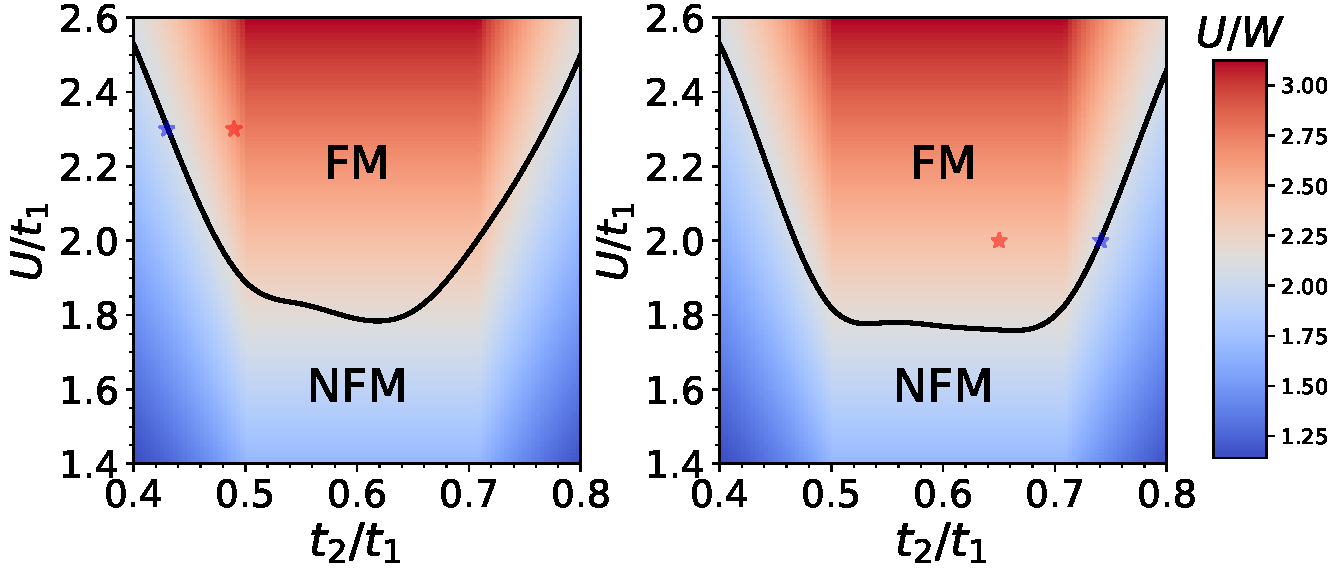
\includegraphics[width=\columnwidth]{phase}
\caption{(Color online) Phase diagram of the quarter-filled (a) Chern Hubbard model and (b) $Z_2$ Hubbard model. The colormap represents the ratio $U/W$ of the lower electron band, where $U$ is the Hubbard interaction strength and $W$ is the lower electron bandwidth. Red stars in (a) and (b) mark the parameters used in Fig. \ref{fmcispectrum} and Fig. \ref{tispectrum}(a), respectively. Blue stars in (a) and (b) mark the parameters used in Fig. \ref{pbcispectrum}. and Fig. \ref{tispectrum}(b), respectively.}
\label{phase}
\end{figure}

\par The phase diagrams of the quarter-filled Chern Hubbard model and $Z_2$ Hubbard model are shown in Fig. \ref{phase}. Here, the colormap represents the ratio of the Hubbard interaction strength $U$ over the lower electron bandwidth $W$. FM denotes the ferromagnetic phase and NFM denotes the non-ferromagnetic phase. As is discussed in Sec. \ref{exact_diag_proj}, the phase boundary is determined as the onset point of $U$ below which negative spin-1 excitation spectra appear. It is clear that a critical Hubbard interaction strength is needed to maintain the ferromagnetically ordered ground state when the electron band has finite nonflatness. This observation is expected as a result from the competition between the kinetic energy and the potential energy of the electrons, as a fully spin-polarized state minimizes the energy of Hubbard interactions but cost more energy when the electron band disperses. An intriguing fact about the phase diagrams is that the phase boundaries always lie near the contour line with $U/W=2.0$.

\subsection{Chern Hubbard model}
\begin{figure}
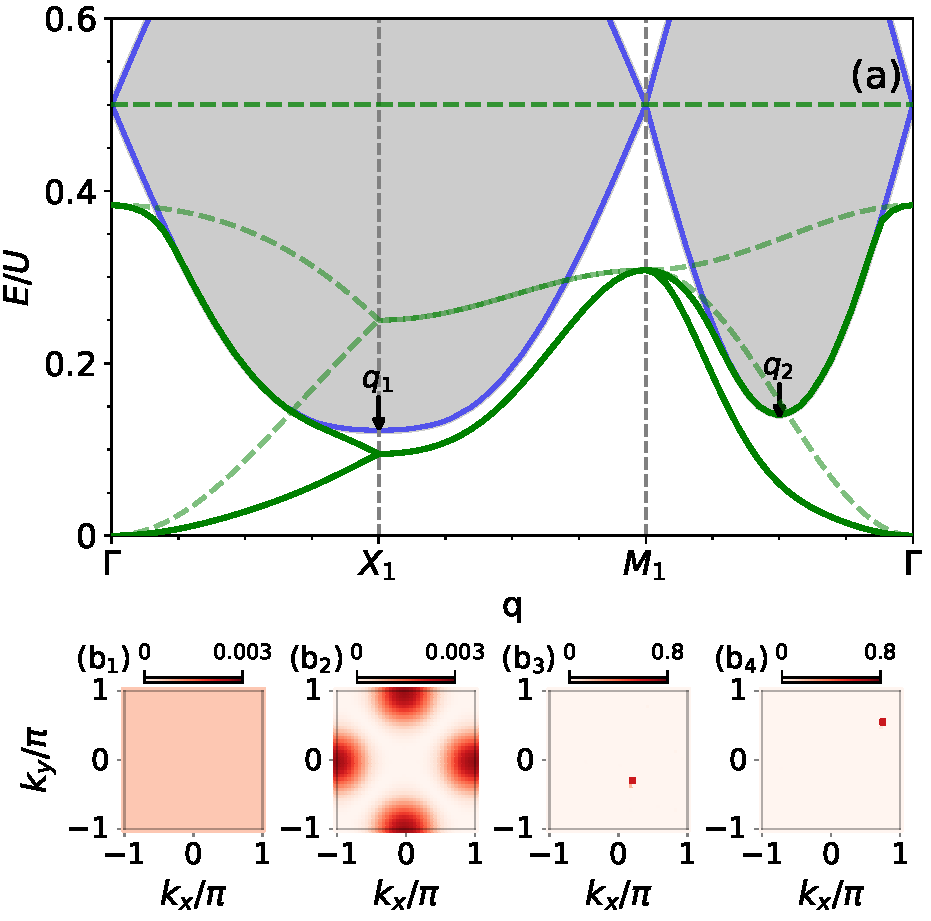
\includegraphics[width=\columnwidth]{fmcispectrum}
\caption{(Color online) (a) Spin-1 excitation spectra of the Chern Hubbard model in the FM phase. Green solid lines denote the spin waves and the grey regions denote the Stoner continuum. Green dashed lines represent the corresponding spectra in the flatband limit. Blue solid lines denote the upper and lower boundaries of the Stoner continuum determined by the split band picture shown in (c). Black arrows mark the local minima of the Stoner continuum. (b) Spectral weights for the lowest four eigen levels of the spin-1 excitation spectra with the center-of-mass momentum $\mathbf{q}=(0,0)$. (c) Illustration of the splitting of the lower electron bands for up spins (blue solid line) and down spins (blue dashed line) in the presence of ferromagnetism of the Chern Hubbard model. Inset shows the positions of the corresponding local maxima (red solid circles) of the spin-up bands and local minima (purple solid circles) of the spin-down bands in the first Brillouin zone. Green arrows denote the corresponding scattering channels of the dips of the Stoner continuum marked in (a). (d) Differences of the spectral weights subtracted by those in the flatband limit for the lowest four eigen levels of the spin-1 excitation spectra with the center-of-mass momentum $\mathbf{q}=(\pi,0)$. The parameters are $t_1=1.0$, $t_2=0.49$ and $U=2.3$.}
\label{fmcispectrum}
\end{figure}

\par To gain a comprehensive understanding of the physics observed above, the spin-1 excitation spectra along a high symmetry path in the first Brillouin zone of the quarter-filled Chern Hubbard model with two different $t_2$ values are plotted in Fig. \ref{cispectrum}(a)-(b) as the green solid lines and the shaded areas. For a comparison, the spectra for those in the corresponding flat-band limit are shown as the green dashed lines as well. Apparently, for both the original model and the flat-band limit model, the spectra consist of two types of modes: the low-lying ones exhibiting well-defined band structures and the high-energy ones forming a continuum. The former are identified as the magnons with an acoustic branch and an optical branch while the latter are identified as the Stoner continuum. At $\Gamma$ point, the acoustic magnon band is gapless, which is the character of a ferromagnetic excitation with the Goldstone mode as the result of the spontaneous spin $SU(2)$ symmetry breaking. Remarkably,

\begin{figure}
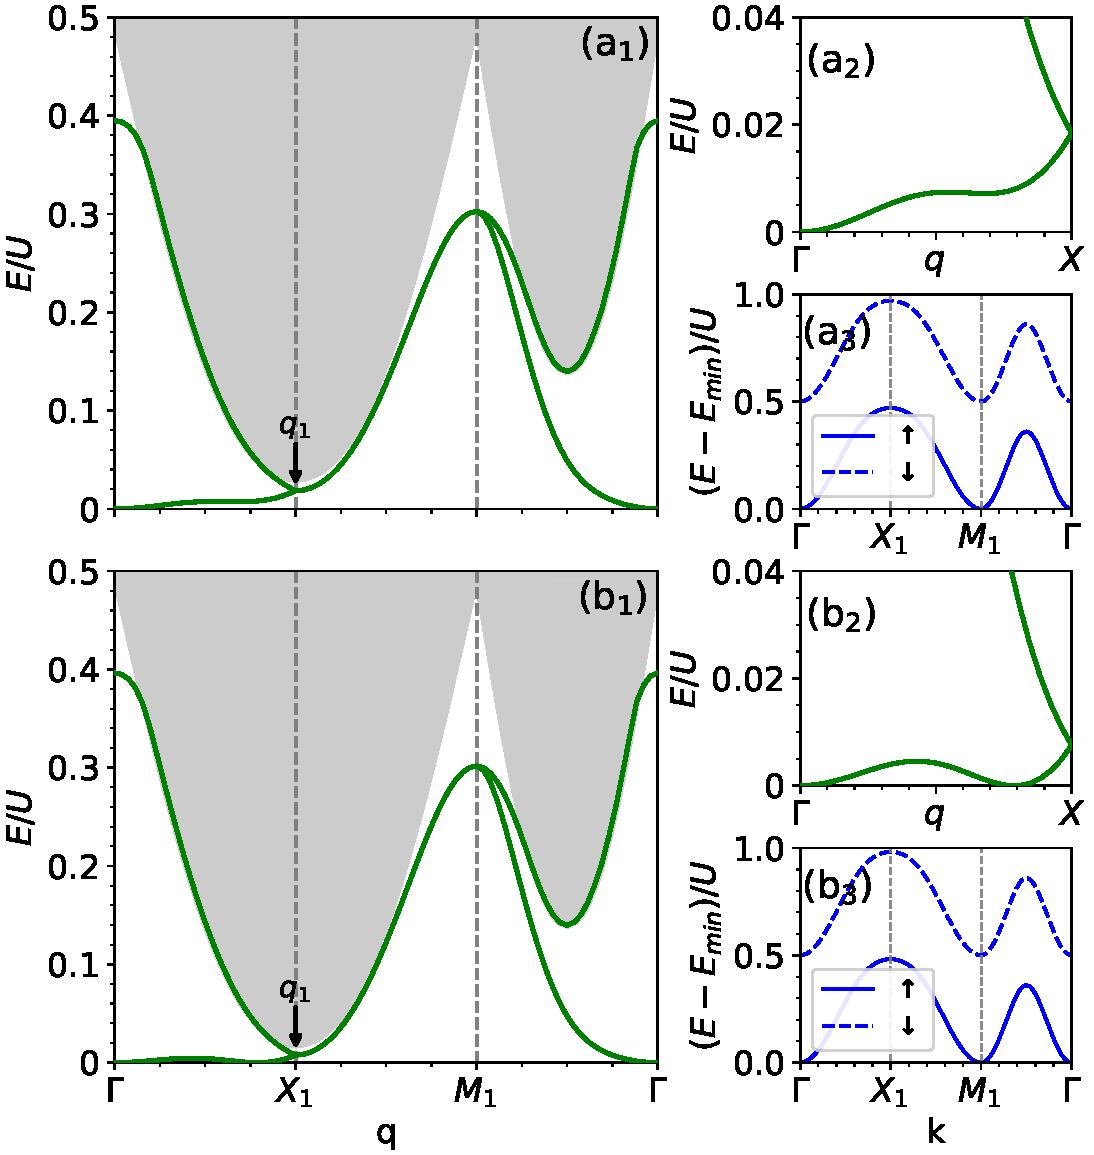
\includegraphics[width=\columnwidth]{pbcispectrum}
\caption{(Color online) (a) Spin-1 excitation spectra of the Chern Hubbard model at the FM/NFM phase boundary. Black arrow marks the minimum of the Stoner continuum. Inset shows its low-energy part along $\Gamma$-$X$ path with an amplified resolution. (b) Illustration of the splitting of the lower electron bands of the Chern Hubbard model. Inset shows the positions of the corresponding local maxima (red solid circles) of the spin-up bands and local minima (purple solid circles) of the spin-down bands in the first Brillouin zone. Green arrows denote the corresponding scattering channels of the minimum of the Stoner continuum marked in (a). The parameters are $t_1=1.0$, $t_2=0.43$ and $U=2.3$.}
\label{pbcispectrum}
\end{figure}

%\par The Hamiltonian has SU(2) spin rotation symmetry. The ferromagnetic ground state breaks SU(2) spin rotation symmetry to U(1) symmetry, and one would therefore expect the presence of a Goldstone mode in the spin-wave excitation spectrum due to spontaneous broken symmetry. We show such a mode at the center of the Brillouin Zone [see Fig.~\ref{fig3}]. The lowest two bands (black solid line and red dashed line) respectively corresponds to the acoustic and optical magnon (spin-wave excitation) bands degenerating along the $X-M$ path in the Brillouin Zone while the higher excitations represent to Stoner continuum in Fig.~\ref{fig3}. $G_{1}(\mathbf{k}_{i},\mathbf{Q})$ dominates the Stoner excitation gap while $G_{2}(\mathbf{k}_{i},\mathbf{k}_{j},\mathbf{Q})$ has very little contribution to the Stoner gap. With the increase of $W/U$, the optical spin-wave excitation is eventually absorbed in the Stoner continuum along the $\Gamma-X$ path in the Brillouin Zone [see Fig. \ref{fig3}(a),(b),(c)]. For $U_{c}=2t_{1}$ ($W/U_{c}=0.414$), there is a critical situation of ferromagnetic ground state, consistent with the theory of Tasaki \cite{Tasaki1} [see Fig.~\ref{fig3}(c)]. When $W/U>W/U_{c}$, the spin-wave excitation appears to be negative somewhere, and the ground state is no longer fully spin-polarized ferromagnetic state.  In order to investigate the effect of the $c$ band to the spin-1 excitation spectrum, we have to consider the case that the $c$ band is assumed as a completely flat-band. In this case, the excitation energies are proportional to the on-site repulsion $U$ instead of the nearest-neighbor hopping energy $t_{1}$ and the boundary of Stoner continuum coalesces into a line [see Fig.~\ref{fig3}(d)]. No matter how small the repulsion $U$ is, the ground state is a fully spin-polarized ferromagnetic state. In contrast to this case, the dispersion of the $c$ band makes the excitation spectrum have the downwarping behavior and gives rise to the phase transition for $U=2t_{1}$ [see Fig.~\ref{fig3}(a),(b),(c)]. The spin-wave excitation spectrum in Fig.~\ref{fig3}(d) is qualitatively similar to the result of the bosonization formalism in ref.~\cite{Doretto}. However, Our result takes into account the effect of the spin-wave interaction in the bosonization formalism. The bosonization formalism neglects the contribution of the nearly flat-band to the spin wave excitation and can't determine what the $W/U$ value is, the ground state is the fully spin-polarized ferromagnetic state.

\subsection{Topological Hubbard model}
\begin{figure}
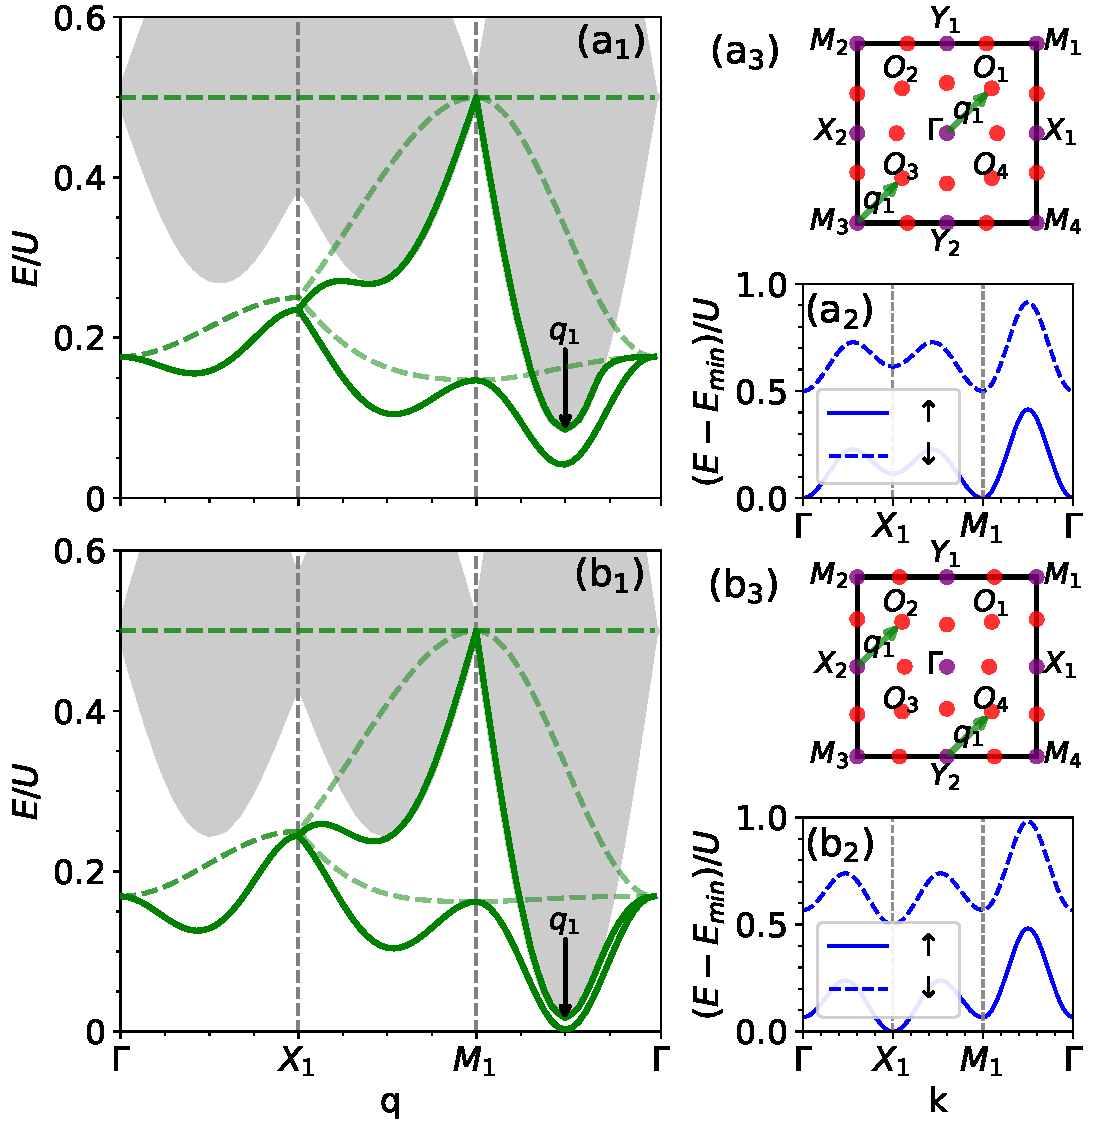
\includegraphics[width=\columnwidth]{tispectrum}
\caption{(Color online) (a) and (b): Spin-1 excitation spectra of the $Z_2$ Hubbard model. Green solid lines denote the spin waves and the grey regions denote the Stoner continuum. Green dashed lines represent the corresponding spectra in the flatband limit. Black arrows mark the minima of the Stoner continuum. (c) and (d): Illustration of the splitting of the lower electron bands of the $Z_2$ Hubbard model. Insets show the positions of the corresponding local maxima (red solid circles) of the spin-up bands and local minima (purple solid circles) of the spin-down bands in the first Brillouin zone. Green arrows denote the corresponding scattering channels of the minima of the Stoner continuum marked in (a) and (b). $t_2=0.65$ for (a) and (c) and $t_2=0.741$ for (b) and (d). Other parameters are fixed at $t_1=1.0$, $U=2.3$.}
\label{tispectrum}
\end{figure}

%\par The spin-1 excitation spectrum of the the ferromagnetic phase of the topological Hubbard model is shown in Fig.~\ref{fig4}. This result indicates that the ground state of the topological Hubbard model is indeed the fully spin-polarized ferromagnetic state due to the fact that the flipping a spin from such state requires a positive energy for $U_{c}>1.82t_{1}$.

%\par Because of the spin-dependent hopping term, only $z$ component of the total spin operator commutes with the Hamiltonian, the symmetry of the Hamiltonian is explicitly broken to U(1) from SU(2) spin rotation symmetry. A Goldstone mode will not exist in the spin-wave excitation spectrum since the ground state has the same symmetry with the Hamiltonian. Since the symmetry is not spontaneously broken, generally, the spin-wave excitations should be gapped [see Fig.~\ref{fig4}]. The low energy excitations consist of two branches of collective modes identified as the spin-wave excitations degenerating along the $\Gamma-X$ path in the Brillouin Zone below the Stoner continuum. There is a critical $U_{c}=1.82t_{1}$ ($W/U_{c}=0.455$) shown in Fig.~\ref{fig4}(c), when $U<U_{c}$, the ferromagnetic ground state vanishes. Interestingly, the Stoner continuums of the Chern and topological Hubbard models are almost the same because their $G_{1}(\mathbf{k}_{i},\mathbf{Q})$ dominating the Stoner excitation gap are equal [see Fig.~\ref{fig3}(b) and Fig.~\ref{fig4}(a)]. As is shown in the Chern hubbard model, the dispersion of the $c$ band also makes the excitation spectrum have the downwarping behavior (while the collective mode (the red dashed line) is partly absorbed in the Stoner continuum) and gives rise to the phase transition for $U=1.82t_{1}$ [see Fig.~\ref{fig4}]. There exist explicit differences from the result of the bosonization formalism in the spin-wave excitation spectrum and it is not clear whether those differences come from the neglected spin-wave interaction in the bosonization formalism.

\section{Summary and discussion}\label{sd}
%\par In summary, we study the ferromagnetic phase in the 1/4-filled nearly flat-band topological Hubbard model on the square lattice in two cases. The spin-1 excitation spectrums of the models are determined by the PED method. In one case, the model is called Chern Hubbard model, whose hopping term is the $\pi$-flux model with nonzero Chern number and nearly flat-band. The model has SU(2) spin rotation symmetry and  breaks time-reversal symmetry. For $ U>U_{c}=2t_{1}$, the ground state is a completely spin-polarized ferromagnetic ground state. The low energy excitations are identified as the acoustic and optical spin-wave excitation, respectively, the high energy excitations, as the Stoner continuum. The spin-wave excitation spectrum is gapless due to spontaneous broken symmetry associated with the Goldstone mode at the center of the Brillouin Zone. In another case, the model is called topological Hubbard model, whose hopping term is the nearly flat-band $\pi$-flux model with nonzero spin Chern number. The model is invariant under time-reversal symmetry and breaks SU(2) to U(1) spin rotation symmetry. For $ U>U_{c}=1.82t_{1}$, the ground state exhibits a completely spin-polarized ferromagnetic ground state and the excitation spectrum is gapped. The low energy excitations consist of two types of collective modes identified as spin-wave excitations below the Stoner continuum.

%\par We have discussed the effects of the nearly flat-band on the excitation spectrum and the phase transition. The nearly band makes the excitation spectrum have the downwarping behavior. If we assume the nearly flat-band as a completely flat-band, the result indicates that the ground state is a fully spin-polarized ferromagnetic state no matter how small the repulsion $U$ is and there is no phase transition. The reason of phase transition is due to the fact that the nearly flat-band is not a completely flat-band. Finally, for the  Chern Hubbard model, our spin-wave excitation spectrum is qualitatively similar to the result of the bosonization formalism in ref.~\cite{Doretto} if the nearly flat-band is assumed as a completely flat-band. However, for topological Hubbard model, there are explicit differences from the result of the bosonization formalism in the spin-wave excitation spectrum and it is not clear whether those differences come from the neglected spin-wave interaction in the bosonization formalism.

\begin{acknowledgments}
\par This work was supported by the National Natural Science Foundation of China (11774152) and National Key Projects for Research and Development of China (Grant No. 2016YFA0300401).
\par X.-F. S. and Z.-L. G. contributed equally to this work.
\end{acknowledgments}

\bibliography{ref}
\end{document}
